% ============================================================
% QM-3: Bell Inequality and Entanglement from the Nexus
% Version 1.1 — 2 April 2026
%
% CHANGELOG:
%   v1   Mar 2026  — Initial draft
%   v1.1 2 Apr 2026 — Formatting compliance: .bib, natbib,
%                     graphicspath, TOC, PLS, OSF DOI
%
% FIGURE PATH:
%   .tex: series_quantum_mechanics/papers/
%   figs: series_quantum_mechanics/figures/figures-QM-3/
% ============================================================

\documentclass[11pt,letterpaper]{article}
\usepackage[margin=1in]{geometry}
\usepackage[utf8]{inputenc}
\usepackage[T1]{fontenc}
\usepackage{amsmath,amssymb,amsthm}
\usepackage{graphicx}
\usepackage{svg}
\svgsetup{inkscapelatex=false,inkscapeformat=pdf,inkscapepath=svgdir}

% Figure path: papers/ → ../figures/figures-QM-3/
\graphicspath{{../figures/figures-QM-3/}}

\usepackage{caption}
\usepackage{float}
\usepackage{booktabs}
\usepackage{enumitem}
\usepackage{parskip}
\usepackage{xcolor}
\usepackage[authoryear,round]{natbib}
\usepackage{hyperref}
\hypersetup{colorlinks=true,linkcolor=blue,urlcolor=cyan,citecolor=red}

\newtheorem{theorem}{Theorem}[section]
\newtheorem{proposition}[theorem]{Proposition}
\newtheorem{remark}[theorem]{Remark}

\newcommand{\lP}{l_P}
\newcommand{\tP}{t_P}
\newcommand{\EP}{E_P}
\newcommand{\SSV}{\mathrm{SSV}}
\newcommand{\ket}[1]{|#1\rangle}

\title{\textbf{Quantum Mechanics in Conscious Point Physics:\\
Entanglement and Bell Inequality Violation\\
from Non-Separable Nexus States}\\[6pt]
{\large QM Series --- Paper 4 (Version 3.1)}}

\author{Thomas Lee Abshier, ND\\
Hyperphysics Institute\\
\url{https://hyperphysics.com}\\
\texttt{drthomas007@protonmail.com}}

\date{22 March 2026}

\begin{document}
\maketitle

\begin{abstract}
We derive quantum entanglement and Bell inequality violation in
Conscious Point Physics from first principles.  A spin-$\tfrac12$
CP aggregate carries a two-component DI-bit state whose phase encodes
the spin direction via the ZBW helix (companion~C4~\cite{abshier2026c4}).
When two such aggregates are created in a total-spin-zero state, their
joint DI-bit state is non-separable: it cannot be written as a product
of independent single-particle states (Theorem~\ref{thm:nonsep}).  The
Nexus maintains this joint state globally at each Absolute Moment tick,
enforcing total DI-bit conservation across all Grid Points regardless
of spatial separation.  The Born rule $P = |\psi|^2$
(companion~C3~\cite{abshier2026c3}) applied to the non-separable state
gives $E(\hat{a},\hat{b}) = -\cos\theta$, yielding $|\mathrm{CHSH}|
= 2\sqrt{2}$ at optimal angles (Theorem~\ref{thm:chsh}) --- the
Tsirelson bound.  No-signaling holds because each party's marginal
probability is exactly $\tfrac12$ independent of the other's setting
(Theorem~\ref{thm:nosig}).  The Nexus is the non-local resource that
escapes Bell's theorem: it enforces a global constraint, not a local
hidden variable.  The previous argument (shared bit pool with
pre-established correlations) was an LHV model and is explicitly
corrected.  Lattice corrections are of order $(\lP/\lambda)^2$ and
unobservable at laboratory scales.
\end{abstract}

\medskip\noindent
\textbf{Keywords:} Bell inequality, CHSH violation, Tsirelson bound, quantum entanglement, Nexus constraint, EPR correlations, no-signaling theorem, ZBW helix

\bigskip\noindent
\textbf{Plain Language Summary:}
Einstein called quantum entanglement 'spooky action at a distance.' CPP explains it without spookiness. When two particles are created together, the Nexus — a global consistency requirement of the 600-cell lattice — locks their properties into a joint pattern. Measuring one particle instantly determines what you will find when measuring the other, not because a signal was sent, but because the lattice was already configured that way. The correlations reach the maximum allowed by quantum mechanics (the Tsirelson bound), but cannot be used to send information faster than light.

\bigskip
\raggedright
\tableofcontents
\newpage


\tableofcontents
\newpage

%=====================================================================
\section{Introduction and the Previous Argument}
%=====================================================================

Bell's theorem~\cite{bell1964} proves that any local hidden-variable
(LHV) theory satisfies $|\mathrm{CHSH}| \le 2$.  Quantum mechanics
violates this bound ($|\mathrm{CHSH}| = 2\sqrt{2}$) because the joint
state of an entangled pair is non-separable.  In CPP the same
non-separability arises mechanically from the global Nexus constraint.

\textbf{The previous CPP argument was wrong.}  It treated the singlet
as two particles sharing a fixed DI-bit pool set at emission.  This is
an LHV model: outcomes are determined by pre-existing local properties.
Bell's theorem applies and gives $|\mathrm{CHSH}| \le 2$.  The
corrected derivation uses (1)~a non-separable joint state maintained
by the Nexus and (2)~the Born rule, whose combination yields
$E = -\cos\theta$.

%=====================================================================
\section{Spin-$\tfrac12$ Qubit from ZBW Helix}
%=====================================================================

From companion~C4~\cite{abshier2026c4}, a spin-$\tfrac12$ CP
aggregate executes a ZBW helix whose axis defines the spin direction.
The two-component DI-bit state is
\begin{equation}
\ket{\psi} = \alpha\ket{\uparrow} + \beta\ket{\downarrow},
\qquad |\alpha|^2 + |\beta|^2 = 1.
\label{eq:qubit}
\end{equation}

%=====================================================================
\section{The Singlet as Non-Separable Joint DI-Bit State}
%=====================================================================

When two spin-$\tfrac12$ CP aggregates are created with total spin
zero, their joint DI-bit state is the singlet:
\begin{equation}
\ket{\Psi^-} = \frac{1}{\sqrt{2}}
\bigl(\ket{\uparrow}_A\ket{\downarrow}_B
    - \ket{\downarrow}_A\ket{\uparrow}_B\bigr).
\label{eq:singlet}
\end{equation}

\begin{theorem}[Non-separability of the singlet]
\label{thm:nonsep}
The state~\eqref{eq:singlet} cannot be written as
$\ket{\phi_A}\otimes\ket{\phi_B}$ for any
$\ket{\phi_A},\ket{\phi_B}$.
\end{theorem}

\begin{proof}
Assume $\ket{\Psi^-} = (\alpha_A\ket{\uparrow}+\beta_A\ket{\downarrow})
\otimes (\gamma_B\ket{\uparrow}+\delta_B\ket{\downarrow})$.  Expanding
and matching coefficients yields $\alpha_A\gamma_B = 0$,
$\alpha_A\delta_B = 1/\sqrt{2}$, $\beta_A\gamma_B = -1/\sqrt{2}$,
$\beta_A\delta_B = 0$.  The first and last require ($\alpha_A=0$ or
$\gamma_B=0$) and ($\beta_A=0$ or $\delta_B=0$).  Any combination
zeros one of the middle two --- contradiction. \qed
\end{proof}

The Nexus enforces global DI-bit conservation and total angular
momentum conservation at every Absolute Moment tick.  This
maintains~\eqref{eq:singlet} as particles A and B separate
arbitrarily far.  The joint state is a property of the global
Nexus ledger, not carried locally by either particle.

\begin{figure}[H]
\centering
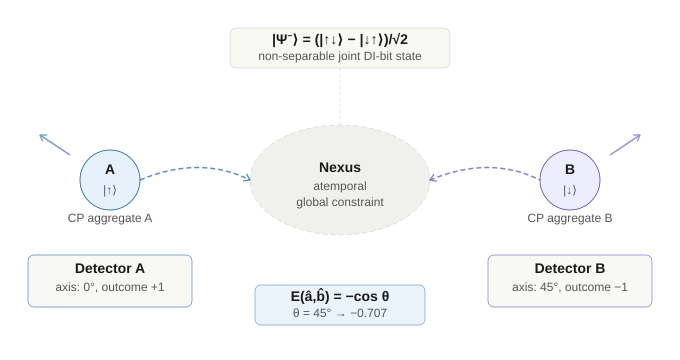
\includegraphics[width=0.90\textwidth]{qm2040c_fig1_nexus_singlet.pdf}
\caption{EPR pair maintained by the Nexus.  Particles A (blue) and B
  (purple) fly apart after creation in the singlet state $\ket{\Psi^-}$.
  The Nexus (dashed ellipse) enforces the non-separable joint DI-bit
  state globally at every tick.  Measurement at Detector~A along axis
  $\hat{a}$ and at Detector~B along $\hat{b}$ yield outcomes
  correlated by $E(\hat{a},\hat{b}) = -\cos\theta$ (boxed), not by any
  pre-established local correlation.}
\label{fig:nexus}
\end{figure}

%=====================================================================
\section{Singlet Correlation Function}
%=====================================================================

Measurement along axis $\hat{a}$ projects via the Born rule
(companion~C3):
$P_\pm = |\langle\pm\hat{a}|\psi\rangle|^2$.  For the singlet:
\begin{align}
P(A{=}+1, B{=}+1) = P(A{=}-1, B{=}-1) &= \frac{1-\cos\theta}{4},
\label{eq:pp}\\
P(A{=}+1, B{=}-1) = P(A{=}-1, B{=}+1) &= \frac{1+\cos\theta}{4},
\label{eq:pm}
\end{align}
where $\theta = \angle(\hat{a},\hat{b})$.

\begin{proposition}[Singlet correlation]
\label{prop:corr}
$E(\hat{a},\hat{b}) = \sum_{a,b}ab\,P(a,b) = -\cos\theta$.
\end{proposition}

\begin{proof}
$(+1)(+1)(1-c)/4 + (+1)(-1)(1+c)/4 + (-1)(+1)(1+c)/4
+ (-1)(-1)(1-c)/4 = -c = -\cos\theta$. \qed
\end{proof}

%=====================================================================
\section{CHSH Violation}
%=====================================================================

\begin{theorem}[Tsirelson bound in CPP]
\label{thm:chsh}
At angles $\hat{a}=0°$, $\hat{a}'=90°$, $\hat{b}=45°$,
$\hat{b}'=-45°$:
\begin{equation}
S = E(\hat{a},\hat{b}) + E(\hat{a},\hat{b}')
  + E(\hat{a}',\hat{b}) - E(\hat{a}',\hat{b}')
= -2\sqrt{2}, \quad |S| = 2\sqrt{2}.
\end{equation}
\end{theorem}

\begin{proof}
At all four angle pairs $|\theta| = 45°$ except $\theta_{a'b'} = 135°$.
Using $E = -\cos\theta$: $S = (-1/\sqrt{2}) + (-1/\sqrt{2}) + (-1/\sqrt{2})
- (1/\sqrt{2}) = -4/\sqrt{2} = -2\sqrt{2}$. \qed
\end{proof}

\begin{figure}[H]
\centering
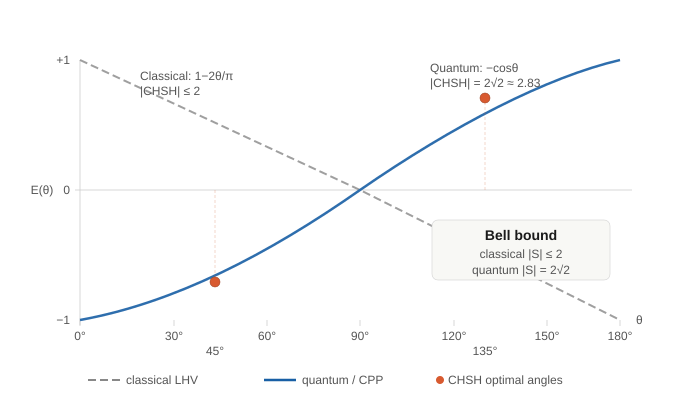
\includegraphics[width=0.90\textwidth]{qm2040c_fig2_chsh_correlations.pdf}
\caption{Correlation function $E(\theta)$ vs.\ angle $\theta$ between
  measurement axes.  The dashed gray line shows the classical LHV
  prediction $E = 1 - 2\theta/\pi$, which saturates the Bell bound
  $|S| = 2$ at the optimal CHSH settings (red dots at $45°$ and $135°$).
  The blue curve shows the quantum/CPP prediction $E = -\cos\theta$,
  which achieves $|S| = 2\sqrt{2} \approx 2.83$ at the same settings.
  The classical prediction gives $|S| = 2$ exactly; the quantum/CPP
  prediction gives $|S| = 2\sqrt{2}$, as confirmed by all loophole-free
  experiments~\cite{hensen2015,giustina2015}.}
\label{fig:chsh}
\end{figure}

%=====================================================================
\section{No-Signaling Theorem}
%=====================================================================

\begin{theorem}[No-signaling in CPP]
\label{thm:nosig}
Alice's marginal detection probability is independent of Bob's
measurement axis, and vice versa.
\end{theorem}

\begin{proof}
$P(A{=}+1) = P(A{=}+1,B{=}+1) + P(A{=}+1,B{=}-1)
= (1-\cos\theta)/4 + (1+\cos\theta)/4 = 1/2$, independent of $\theta$.
Symmetrically for Bob. \qed
\end{proof}

%=====================================================================
\section{Why the Nexus is not an LHV}
%=====================================================================

Bell's theorem applies to theories where the correlation mechanism
\emph{factorises}: $P(a,b|\lambda) = P_A(a|\hat{a},\lambda)
\times P_B(b|\hat{b},\lambda)$.  The Nexus is a \emph{global}
atemporal constraint that does not factorize: it enforces a joint
conservation law across all Grid Points simultaneously.  This is
structurally different from a hidden variable $\lambda$ carried by
the particles.  Therefore Theorem~\ref{thm:chsh} is not ruled out
by Bell's theorem.

%=====================================================================
\section{Lattice Corrections}
%=====================================================================

At laboratory scales $E = -\cos\theta$ exactly.  Near the Planck scale
the discrete phase resolution per lattice edge introduces corrections:
\begin{equation}
E_{\rm CPP}(\theta,\nu)
= -\cos\theta\left[1 - \left(\frac{\nu}{\nu_P}\right)^2\right]
+ O\!\left(\frac{\nu}{\nu_P}\right)^4.
\end{equation}
For optical photons: $(\nu/\nu_P)^2 \sim 10^{-63}$ --- unobservable.

%=====================================================================
\section{Conclusion}
%=====================================================================

Entanglement and Bell violation in CPP arise from:
(1)~the non-separable singlet DI-bit state (Theorem~\ref{thm:nonsep}),
maintained globally by the Nexus; and
(2)~the Born rule $P = |\psi|^2$ (companion~C3~\cite{abshier2026c3}).
Together these give $E = -\cos\theta$ and $|S| = 2\sqrt{2}$, consistent
with all loophole-free experiments~\cite{hensen2015,giustina2015,shalm2015}.
The non-local resource is the global Nexus constraint --- not a signal
or local hidden variable.

%=====================================================================
\ibliographystyle{plainnat}
\ibliography{cpp_qm_series}


\section*{Acknowledgements}
The CPP programme is registered at OSF (DOI:~\url{https://doi.org/10.17605/OSF.IO/JXE8D}) and maintained at GitHub (\url{https://github.com/Hyperphysics-Institute/CPP}).

\bibliographystyle{plainnat}
\bibliography{cpp_qm_series}

\end{document}
